\chapter{Grundriss Prototyp} 
	In den bisherigen Prototypen wurde die Migration auf das Modulsystem von Java behandelt. Jedoch ist das Problem des dynamischen Ladens und Auswechselns von Plugins während der Laufzeit nicht thematisiert worden. Dieser Prototyp erarbeitet mithilfe der neu eingeführten Konzepte des Modulsystem einen möglichen Grundriss für die dynamischen Umsetzung eines Plugin-Systems. Hierfür werden die Module, die Modulschichten sowie der Java \textit{Service-Lader} eingesetzt.

\section{Anforderungen} 
	Zurzeit können die Plugins in die laufende Applikation integriert werden. Dazu wird die eingebaute Funktion des Klassenladers genutzt. Der Klassenlader kann neue Plugin-Code in das System integriert, jedoch können die geladenen Plugins im Nachhinein nicht mehr entladen werden. Dementsprechend soll erforscht werden, ob mithilfe des Modulsystem eine Lösung für das bestehende Problem gefunden werden kann. Für die Lösung soll ein Grundriss Prototyp entstehen, welcher das dynamische Laden und Entladen der Plugins skizziert. Der Prototyp soll keine lauffähige Logik von \textsc{Renew} oder \textsc{Mulan} umsetzen, sondern das Laden und Entladen von Java-Code darstellen.

\section{Spezifikation} 
	Für die Umsetzung wird der aktuelle Zustand von \textsc{Renew} begutachtet und zuvor erarbeitete, aber nicht integrierte Lösungsansätze zusammengefasst. Die nachfolgende Anfertigung des konzeptionellen Grundrisses erstellt eine Modulschicht per Plugin und verknüpft die Plugins mit einander über die Schichtendelegation sowie die \textit{Service-Lader} Instanz. Das Ergebnis stellt eine Fassade dar, die nachfolgend als ein Grundriss implementiert und ausgewertet wird.

\section{Entwurf} \label{sec:entwurf}
	Die grundlegende Idee der Modulschichten und des \textit{Service-Laders} wurde im Kapitel \ref{sec:module_layers} und \ref{sec:servLoad} diskutiert. Mithilfe der Module, Modulschichten und des \textit{Service-Laders} wird in diesem Abschnitt ein Grundriss des möglichen Einsatzes im Plugin-Management vorgestellt.\bigbreak

	Das zentrale Problem der zurzeit betriebenen Umsetzung ist das monolithische Verhalten der Plugins, die sich den gleichen Klassenraum teilen, direkte Zugriffe durchführen und während der Laufzeit nicht voneinander getrennt werden können. Denn die \textsc{Renew}-Plugins sind an den Plugin-Klassenlader gebunden und dürfen laut der Java Plattform diesen nicht mehr verlassen. \newline
	Um die Plugins aus der Applikation endgültig zu entfernen, müssen die Plugins auf separate Klassenlader aufgeteilt und betrieben werden. Durch den Einsatz von mehreren Klassenlader kann die Referenz auf einen bestimmten Klassenlader Objekt, welches ein Plugin in sich trägt, gelöscht oder neue belegt werden. Somit ist das ehemalige Klassenlader-Objekt nicht mehr erreichbar und wird von dem \textit{Garbage Collector} aus dem Speicher entfernt.\bigbreak 

	Wie bereits in den Grundlagen Kapitel \ref{cha:Grundlagen} behandelt, sind die zur Verfügung gestellten Klassenlader hierarchisch aufgebaut, arbeiten nach dem \textit{Parent First} Delegationsprinzip und können die Anfrage nur an einen übergeordneten Klassenlader delegieren. Dementsprechend fehlt dem Klassenlader-System die Integration der verzweigten Delegation sowie die organisierte Kommunikation zwischen einer variablen Anzahl an Klassenlader, die für das Plugin-System eine große Rolle spielen.\newline
	Mit der Integration der Module sowie Modulschichten in die Java Plattform, sollen die angesprochenen Probleme adressiert und gelöst werden. Aus diesem Grund kümmert sich das Modulsystem von Java um die Authentizität sowie Integrität des Modulinhalts und führt zusätzlich das Konzept der Modulschichten eine, welches das Verwalten der System-Modulbausteine übernimmt und den genauen Aufenthaltsort jedes Moduls sowie seiner zuständigen Verwaltungsinstanz überblickt. Da die \textsc{Renew}-Plugins als Module umgesetzt worden sind, genießen sie die Eigenschaften der Module sowie die Unterstützung des Modulsystems.\newline
	Die Verwaltung des Plugin-Inhalts und dessen Abhängigkeiten werden über die expliziten Schnittstellen angegeben und über eine Konfiguration, die einen Teil der Modulschicht darstellt, validiert. Die Konfiguration erstellt einen Plugin-Abhängigkeitsgraphen, der aus einer gegebenen Verzeichnis Menge einem auserwählten Wurzel-Plugin und einer optionalen Anzahl von untergeordneten Konfigurationen Plugin-Beziehungen herstellt. Die Konfiguration validiert und stellt sicher, dass alle benötigten Abhängigkeiten gefunden und aufgelöst werden, keine Zyklen durch das hinzufügen neuer Plugins sowie Bibliothek entstehen und jedes Plugin sowie jede Bibliothek eindeutig jeder Suchanfrage zugeordnet werden kann. Somit überblickt die Konfiguration das Modulkonstellation und den Zustand ihre Schicht sowie der darunterliegenden Modulschichten. Dies hat zur Folge, dass Plugins und Drittanbieter-Bibliotheken nur einmal in der Schicht-Konfiguration auftreten können und verhindert das Überladen von bestehender Funktionalität.\newline
	Die elastische Konfigurationseinstellung und die globale Konsistenz der modularen Applikation ermöglichen eine verzweigte Delegation der Suchanfrage an bekannte Modulschichten und dessen Plugin-Module, die zuvor validiert und in die Applikation eingebettet worden sind. Somit kennt die Applikation alle Plugins sowie die dazugehörige Bibliotheken und kann die Suchanfrage an die entsprechende Schicht weiterleiten, ohne ein Sicherheitsrisiko einzugehen.\newline
	Die neu eingeführte verzweigte Delegation spielt eine große Rolle für das Plugin Konzept, denn die Plugins erweitern und werden von anderen zahlreichen Plugins erweitert. Die dynamische Zusammensetzung der Plugins kann ohne Struktur und umfassende Sicherheitsmechanismen nicht mängelfrei in einem großen System bestehen. Dementsprechend muss das erweiternde Plugin von unerwarteten äußeren Einflüssen geschützt werden und vor dem Einbinden in die Applikation eine valide Strukturintegration nachweisen. Die genannten Anforderungen werden bestens von den Modulen und den Modulschichten abgedeckt, die mit der zusätzlichen verzweigten Delegation neue Möglichkeiten der Java Plattform  und somit auch \textsc{Renew} bieten.\bigbreak

	Im Folgenden wird ein Prototyp vorgestellt, der ein Plugin System simuliert, welches aus Modulen sowie  Modulschichten besteht und als ein Grundriss für die mögliche Umsetzung der nächsten \textsc{Renew} Version dienen könnte. \bigbreak
			
	\begin{figure}[t]
		   \centering
		   \captionsetup{justification=centering}
		   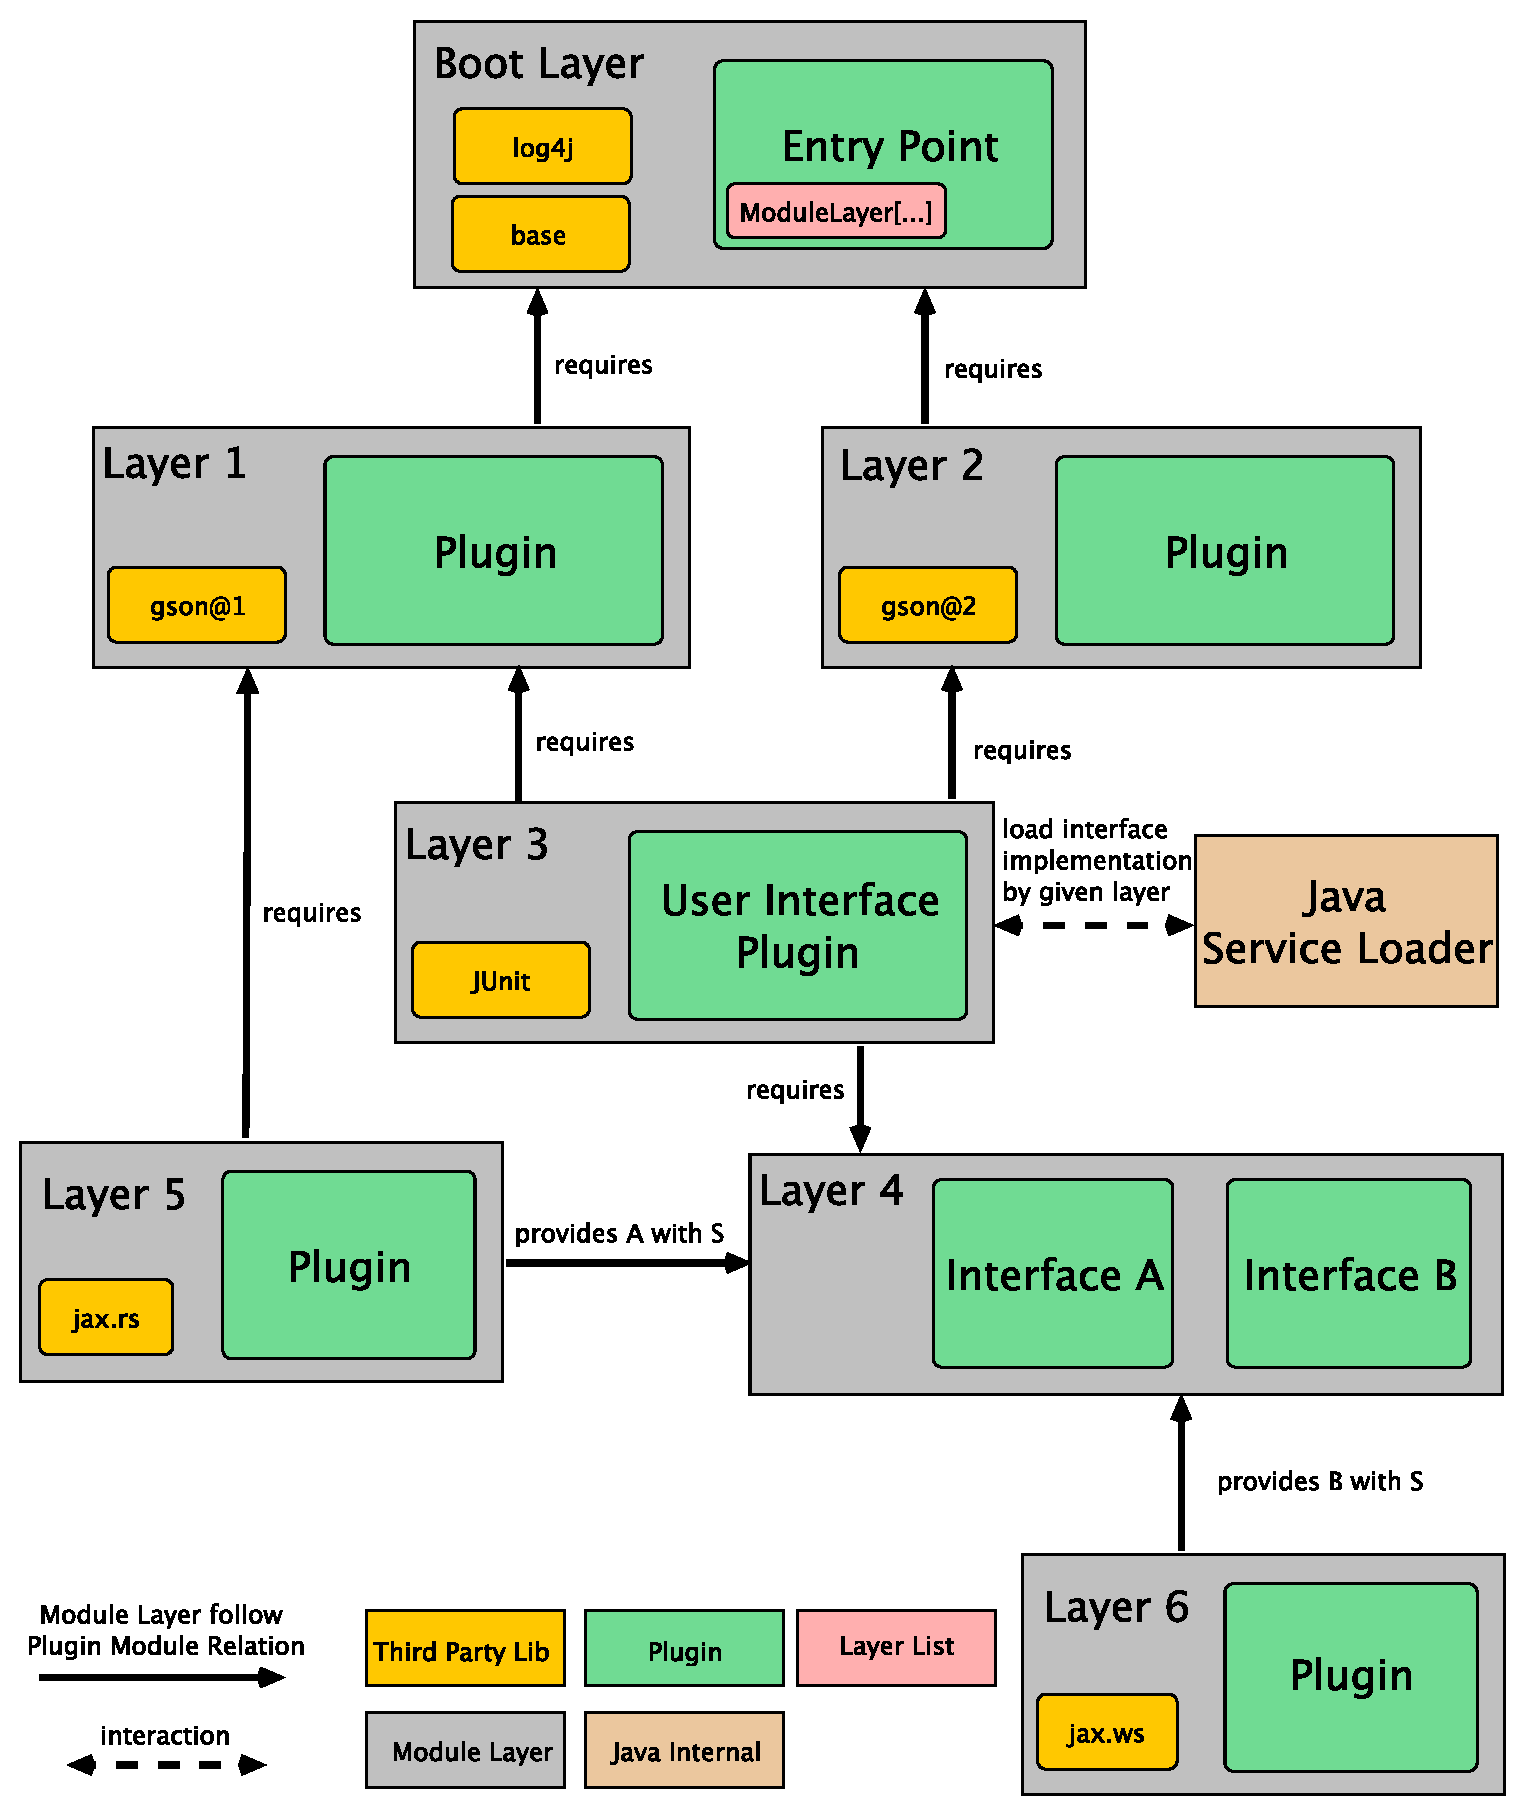
\includegraphics[width=0.8\textwidth]{material/images/ModulLayerDepsDraw.pdf}
		   \caption{Grundriss einer möglichen Plugin-Architektur auf Basis der Modulschichten}
		   \label{fig:ModSchichtKonzept}
	\end{figure}
\newpage	
	Die Abbildung \ref{fig:ModSchichtKonzept} visualisiert den Grundriss. Ganz Oben in der Schichten Hierarchie befindet sich die \textit{Boot-Schicht}, diese enthält die von Java zur Verfügung gestellten Module sowie den Einstiegspunkt der Applikation. Der Einstiegspunkt der Applikation erstellt und verwaltet die Plugins über die zur Laufzeit erstellten Modulschichten. Die darunterliegenden Schichten \textit{eins} und \textit{zwei} stellen zwei unterschiedliche Plugin Funktionalitäten dar, die dieselbe Bibliothek \textit{gson} in unterschiedlicher Version nutzen und die Möglichkeit des parallelen Betriebs illustrieren. Die Modulschicht \textit{drei} baut auf der \textit{zweiten} und \textit{dritten} Modulschichten auf und benötigt dessen Funktionalität für die eignen Implementation. Zum Beispiel könnte es die Funktion des \textit{GUI}-Plugins darstellen, die die \textit{Util} sowie \textit{WindowManagment} Plugins aus der zweiten sowie dritten Modulschicht anfordert. Dementsprechend kann ein Plugin mithilfe der Modulschichten zwei oder mehr übergeordnete Schichten referenziert und auf ihre Funktionalität Konfliktfrei zugreifen.\newline
	Da das \textit{Gui}-Plugin nicht auf allen \textsc{Renew}-Plugins aufbaut, sondern diese lediglich koordiniert, muss die parallel entstehende Logik aus der Schicht \textit{fünf} für das \textit{Gui}-Plugin zugänglich gemacht werden. Dies wird mithilfe des Java \textit{Service-Laders} umgesetzt, der für ein gegebenes Schnittstellen Modul alle zugänglichen Implementationen erfasst und als ein Dienst für die Ausführung dem \textit{Gui}-Plugin anbietet.\bigbreak

\section{Umsetzung}\label{sec:umsetzung}

% section umsetzung (end)
\section{Evaluation}

